% !TEX root = holder_file.tex
\chapter{Preliminaries}

\label{ch: basics}
%----------  section ------------
\section{What Is a Derivative}



\begin{tcolorbox}
	%[colback={red!150!brown!20},coltitle={purple}]
	[colback=Pastel Blue]
	\begin{definition}
	A derivative is a type of financial contract whose value is determined by the value of an underlying asset, group of assets, or benchmark.
	\end{definition}
\end{tcolorbox}

 \noindent A derivative is a contract between two or more parties that can be traded on an over-the-counter (OTC) or exchange . These contracts can be utilized to transact variety of assets and come with their own set of risks. Derivatives prices are determined by fluctuations in the underlying asset. These financial securities are commonly used to gain access to specific markets and may be traded to hedge against risk. \\
 Derivatives can be employed for a position  hedging or speculate upon that direction of an underlying asset, or provide leverage to holdings. These assets are most often traded on over-the-counter (OTC) or exchanges and bought via brokerages. 

\section{Exchange-Traded Market}

\begin{tcolorbox}
	%[colback={red!150!brown!20},coltitle={purple}]
	[colback=Pastel Blue]
	\begin{definition}
		A derivatives exchange is a market in which people buy and sell formalized contracts that the exchange has defined.
	\end{definition}
\end{tcolorbox}

 \noindent Because of the advantages of having over over-the-counter (OTC) derivatives, exchange-traded derivatives have gained popularity. Standardization, liquidity, and the elimination of default risk are among the advantages.\\
 
 Futures and options have been two of the most widely traded ETFs. ETFs can be utilized to hedge exposure and speculate on a broad range of financial securities, including goods, stocks, currencies, and even rate of interest.
\section{Over-The-Counter Markets}

\begin{tcolorbox}
	%[colback={red!150!brown!20},coltitle={purple}]
	[colback=Pastel Blue]
	\begin{definition}
		 It is a network of dealers connected by phone and computer.
	\end{definition}
\end{tcolorbox}

\noindent Derivatives are not always traded on exchanges. In terms of total trading volume, the over-the-counter market has overtaken the exchange-traded market as a significant substitute for exchanges. It is a dealer network that is connected via phone and computer. Typically, trades are conducted over the phone between two financial institutions or between an institution and one of its clients (typically a corporate treasurer or fund manager). For the instruments that are traded more often, financial institutions frequently serve as market makers. As a result, they are constantly ready to provide both an offer price and a bid price (a price at which they are willing to purchase) (a price at which they are prepared to sell).
\section{Forward Contracts}
\noindent A forward contract is a rather straightforward derivative. 
\begin{tcolorbox}
	%[colback={red!150!brown!20},coltitle={purple}]
	[colback=Pastel Blue]
	\begin{definition}
		It is an agreement to purchase or sell a particular item at a specific price in the future.
	\end{definition}
\end{tcolorbox}
 \noindent A spot contract, which is a commitment to buy or sell an asset today, can be contrasted with it. In the over-the-counter market, forward contracts are traded, typically between two financial institutions or between a financial institution and one of its clients.
\section{Future Contracts}
\noindent A futures contract, like a forward contract, is an agreement between two parties to buy or sell an item at a certain price and time in the future. Futures contracts, in contrast to forward contracts, are often traded on an exchange. The exchange provides a few standardized aspects of the contract in order to facilitate trade. The exchange also offers a system that gives the two parties a guarantee that the contract will be upheld because the two parties to the contract are not necessarily acquainted.
\section{Types of Traders}
\noindent Markets for derivatives have achieved extraordinary success. The key reason is that they have a large amount of liquidity and have drawn many different kinds of traders.
Finding someone who is willing to take the other side of a contract is typically not an issue when an investor wants to take one side.
Hedgers, speculators, and arbitrageurs are the three main types of traders. Hedgers can lower their risk from probable future changes in a market variable by using derivatives. They are used by speculators to wager on the potential course of a market variable. To guarantee a profit, arbitrageurs take offsetting bets in two or more securities.
\subsection{Hedgers}

\begin{tcolorbox}
	%[colback={red!150!brown!20},coltitle={purple}]
	[colback=Pastel Blue]
	\begin{definition}
		A hedge is an expenditure  with the goal of lowering the risk of unfavorable changes in an asset's price. A hedge often entails taking an opposite or offsetting stake in a connected security.
	\end{definition}
\end{tcolorbox}


\subsection{Speculators}

\begin{tcolorbox}
	%[colback={red!150!brown!20},coltitle={purple}]
	[colback=Pastel Blue]
	\begin{definition}
		A speculator tries to outperform conventional longer-term investors by using tactics and often a shorter time horizon.
	\end{definition}
\end{tcolorbox}

\noindent Speculators assume risk in the hopes of earning profits that are significant enough to outweigh the risk, particularly when predicting future price changes.
\subsection{Arbitrageurs}

\begin{tcolorbox}
	%[colback={red!150!brown!20},coltitle={purple}]
	[colback=Pastel Blue]
	\begin{definition}
		An investor who makes an effort to capitalize on market inefficiencies is known as an arbitrageur.
	\end{definition}
\end{tcolorbox}

\noindent Prices, dividends, regulations, or any other component of the markets may be affected by these inefficiencies. Arbitrage in terms of pricing occurs most frequently.
\section{Options}
\noindent Both on exchanges and in the over-the-counter market, options are exchanged. Two different options are available.
\subsection{Call Options}

\begin{tcolorbox}
	%[colback={red!150!brown!20},coltitle={purple}]
	[colback=Pastel Blue]
	\begin{definition}
		Financial contracts known as call options grant the option buyer the right, but not the commitment, to purchase a stock, bond, commodity, or other asset or instrument at a particular price within a predetermined time window. 
	\end{definition}
\end{tcolorbox}

\noindent The underlying asset is a stock, bond, or product. When the value of the underlying asset rises, the call buyer makes money.
\subsection{Put Options}

\begin{tcolorbox}
	%[colback={red!150!brown!20},coltitle={purple}]
	[colback=Pastel Blue]
	\begin{definition}
		The contract known as a put option (or "put") grants the option purchaser the power, but not the duty, to sell—or sell short—a set amount of the underlying asset at a specified price within a given time span.
	\end{definition}
\end{tcolorbox}

\noindent The striking price is the predetermined price at which the buyer of the put option may sell the underlying security.
\subsection{Option Payoff diagram}

\begin{figure}[!htb]
	\begin{minipage}[l]{0.5\linewidth}
		\begin{center}
			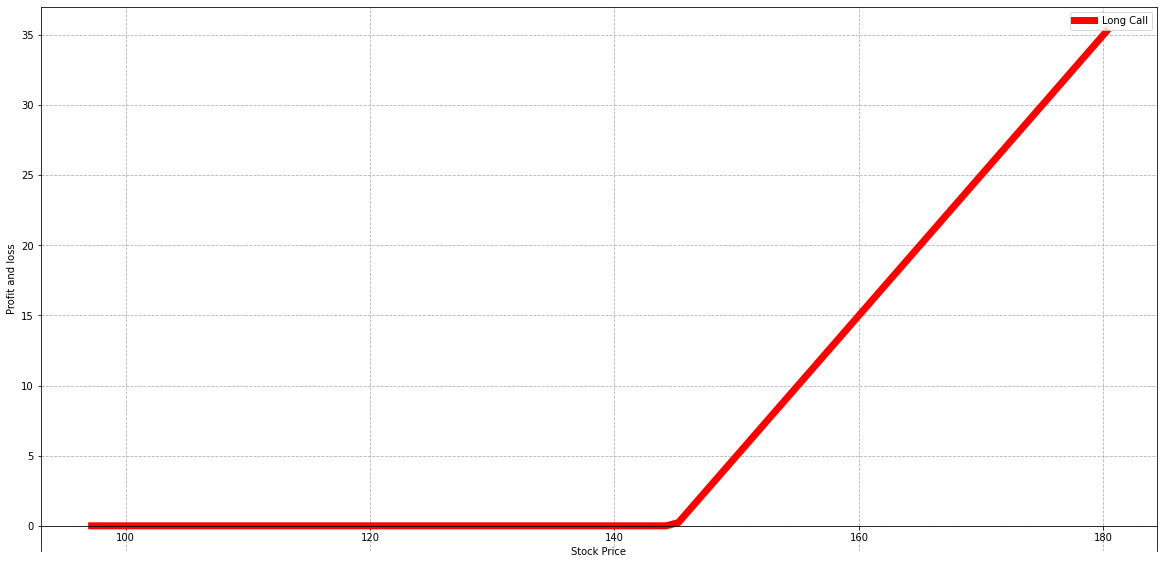
\includegraphics[width=1\textwidth]{Long_call}
		\end{center}
	\end{minipage}
	\hfill
	\begin{minipage}[r]{0.5\linewidth}
		\begin{center}
			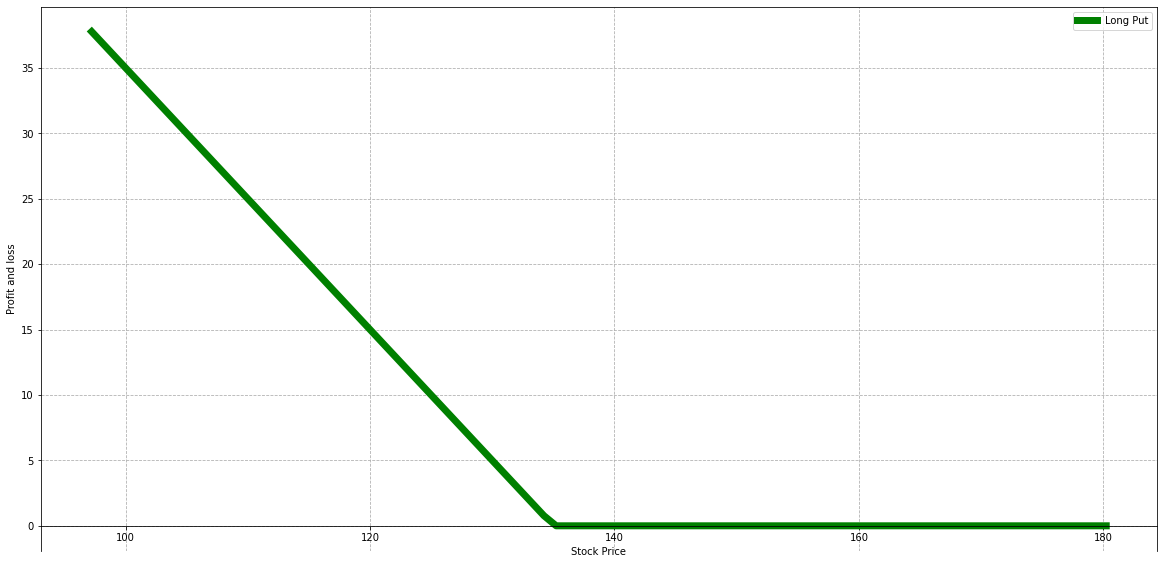
\includegraphics[width=1\textwidth]{Long_put}
		\end{center}
	\end{minipage}
	\caption{ Long Position}
\end{figure}

\begin{figure}[!htb]
	\begin{minipage}[l]{0.5\linewidth}
		\begin{center}
			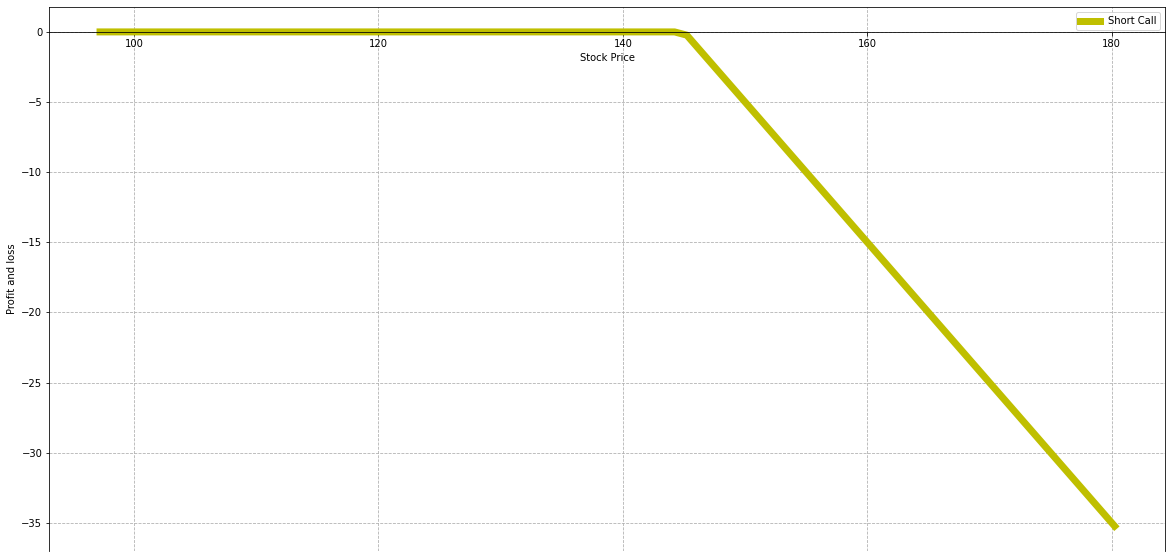
\includegraphics[width=1\textwidth]{Short_call}
		\end{center}
	\end{minipage}
	\hfill
	\begin{minipage}[r]{0.5\linewidth}
		\begin{center}
			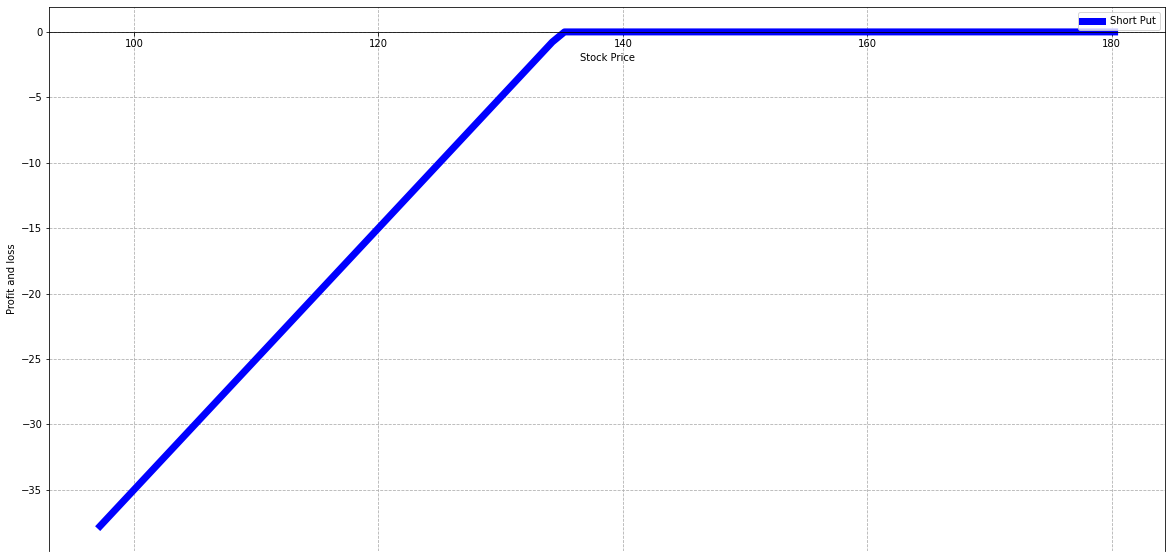
\includegraphics[width=1\textwidth]{Short_put}
		\end{center}
	\end{minipage}
	\caption{ Short Position}
\end{figure}

A put option is a contract that is agreed between the writer or seller and the holder, or buyer. The buyer has the option, but not the responsibility, to sell the underlying security at the striking price and on the termination date. The asset is regarded as the buyer. The contract is guaranteed by the seller, who, upon request, agrees to purchase the asset at the strike price on the expiration date.
This is specifically a European put. In contrast, an American put allows the holder to exercise the option at any time up until the expiration date. We will only consider European choices for the time being.
The call option and put option are presented individually in these diagrams based on their relative positions.   

\subsection{European and American Options}
A contract's price is referred to as the exercise price or strike price, and its date as the expiration date or maturity. Up until the expiration date, American options can be exercised whenever you want. Only the expiration date itself is a valid date for exercising European options. American options make up the majority of those traded on exchanges. One contract on the exchange-traded equity option market typically entails the purchase or sale of 100 shares. In general, European options are simpler to analyze than American options, and many of the characteristics of an American option can be inferred from those of its European equivalent.

\subsection{Exotic and Path Dependent Options}
A path dependent option is an exotic option whose value is influenced by the underlying asset's journey as well as its price across all or a portion of the option's life. Path-dependent options come in a variety of forms, such as Asian, Chooser, Lookback, and Barrier options.\\
The right, but not the responsibility, to buy or sell an underlying asset at a particular price, known as the strike, before or at the expiration date is provided by all options. At the beginning of the contract, options specify the strike price and expiration date. Profitability is often determined by comparing the current market price of the underlying asset to the strike price. However, the price that is utilized to calculate profitability in a path dependent option can change. Profitability may be determined, for instance, by an average price or a high or low price.


\subsection{Barrier options}
A barrier option specifies a second price in contrast to the strike price, the
barrier. Situationally, the barrier may work to activate the choice or invalidate it.
upon the kind. If the barrier price is crossed in the case of a "knock-out" barrier,
The choice loses all value. The situation with a "knock-in" barrier is the
An alternative is presented.
In all likelihood, the cost of a knockout type + the cost of a knockin type
equivalent to the cost of a standard European choice. This suggests that the cost
is always lower than that of its European counterpart for a barrier choice. Their
One benefit of a barrier option is its lower cost.

\section{Put-Call Parity}

\begin{tcolorbox}
	%[colback={red!150!brown!20},coltitle={purple}]
	[colback=Pastel Blue]
	\begin{definition}
		The value of a European call (C) with a specific exercise price (K) and exercise date (T) can be calculated from the value of a European put (P) with the same exercise price and date, and vice versa, if S represents the stock price of a non-dividend paying stock. Put-Call Parity refers to this relationship between the underlying asset and its options.
	\end{definition}
\end{tcolorbox}

$$P+S=C+k\exp[-rT+rt]$$

\noindent For European options, there is a notion known as put-call parity. As they have the same underlying asset, strike price, and expiration date, these options are considered to be of the same class. American options, which can be exercised at any time before the expiration date, are exempt from this rule.

\noindent According to put-call parity, having a short European put and a long European call of the same class at the same time will produce the same return as holding a single forward contract on the same underlying asset, with the same expiration and a forward price equal to the option's strike price.
\section{Risk-Neutral Valuation}
A probability measure called a risk neutral measure is employed in mathematical finance to help with the valuation of derivatives and other financial instruments. In order to determine the accurate price for a given asset, investors must take into account risk neutral measures, which provide a mathematical interpretation of the market's overall risk aversion.

Equilibrium measures and comparable martingale measures are other names for risk neutral measures. 
\section{Stochastic Process}
Stochastic is a technical term meaning random. A system that changes over time while being subject to random fluctuations is said to be in a stochastic process. Such a system can be explained by creating a family of random variables, $(X,t)$,where X, t represents the aspect of the system that is of interest at time t. For instance, X, t might represent the quantity of clients waiting in a line at time t. Customers will come and go as time goes on, changing the value of X, t. Any value in a subset of 0, 1, 2,..., and t at any time take one of those values. $(-\infty,\infty)$, from the endless past to the endless future.
\section{\ito Lemma}
The cost of a stock option depends on the time and price of the underlying stock. In a broader sense, we might state that the price of any derivative depends on both time and the stochastic variables that underlie the derivative. Therefore, a serious student of derivatives must develop some knowledge of how stochastic function behave. Ito's lemma is a significant finding in this field that was made by mathematician K. Ito in. Assume that a variable's value x follows the Ito procedure.
\[dx=a(x,t)dt+b(x,t)dz\]
where a and b are functions of x and t and dz is a weiner process. Drift and variation rates for the variable x are a and?2, respectively. A function G of x and t follows the process, according to Ito's lemma.
\[dG=(\frac{\delta G}{\delta x}a+\frac{\delta G}{\delta t}+\frac{1}{2}\frac{\delta^2 G}{\delta x^2}b^2)dt+\frac{\delta G}{\delta x}bdz\]
where the dz is the same Wiener process. Thus, G also follows an
Ito process, with a drift rate of
\[(\frac{\delta G}{\delta x}a+\frac{\delta G}{\delta t}+\frac{1}{2}\frac{\delta^2 G}{\delta x^2}b^2)\]
and a variance rate of
\[(\frac{\delta G}{\delta x})^2b\]
It is outside the purview of this work to provide an exhaustive proof of Ito's lemma. In the chapter's appendix, we demonstrate how the lemma can be seen as an extension of well-known differential calculus results. \\
We had suggested earlier that
\[dS=\mu S dt+\sigma S dZ\]
with $\mu$ and $\sigma$ constant, is a reasonable model of stock price movements. From Ito's
lemma, it follows that the process followed by a function G of S and t is
\[dG=(\frac{\delta G}{\delta S}\mu S+\frac{\delta G}{\delta t}+\frac{1}{2}\frac{\delta^2 G}{\delta S^2}\sigma^2 S^2)dt+\frac{\delta G}{\delta S}\sigma S dz\]
Be aware that the same underlying source of uncertainty, dz, has an impact on both S and G.
This demonstrates the significance of this in the Black-Scholes-Merton findings derivation.
\section{The Black-Scholes Model}
\subsection{ Introduction}
\noindent A key idea in contemporary finance theory is the Black-Scholes model, commonly referred to as the Black-Scholes-Merton (bf BSM) model. This mathematical formula calculates the potential value of derivatives based on other financial instruments while taking other risk variables and the impact of time into account. It was created in 1973 and is currently regarded as one of the best methods for determining the price of an options contract.
\subsection{ Assumptions}
\noindent The Black-Scholes model makes certain assumptions:\\
\begin{itemize}
	\item The stock price follows the process equation \ref{eq:gmb} with $\mu$ and $\sigma$ constant.
	\item The short selling of securities with full use of proceeds is permitted.
	\item There are no transaction costs or taxes. All securities are perfectly divisible.
	\item There are no dividends during the life of the derivative.
	\item There are no riskless arbitrage opportunities.
	\item Security trading is continuous.
	\item The risk-free rate of interest r, is constant and the same for all maturities.
	\item The option is \emph{European} and can only be exercised at expiration.
\end{itemize}
Although the original Black-Scholes model did not take into account the impacts of dividends paid throughout the option's life, the model is routinely modified to account for dividends by calculating the value of the underlying stock as of the ex-dividend date. Many option-selling market makers also alter the model to take into consideration the impact of options that can be exercised prior to expiration.
\subsection{ Methodology}
\noindent We assume that the stock price process is
\begin{equation}
	dS=\mu S d t+\sigma SdW 
	\label{eq:gmb}
\end{equation}
where $\sigma$ is the volatility, $\mu$ is risk free interest rate and $dW$ is winner process.\\[2mm]
Suppose that $C(S;t)$ be the value of an European option. To derive the {\bf BSM} model, we construct a portfolio of one long option position and a short position in some
quantity $\Delta$ of the underlying:
$$
\Pi=C(S, t)+\Delta S
$$
Over the time interval $d t$ the gain in the value of the portfolio is $t$ is
$$
d \Pi=d C(S, t)+\Delta d S
$$
i.e.
$$
d \Pi=\left(\frac{\partial C}{\partial t} d t+\mu S \frac{\partial C}{\partial S}+\frac{1}{2} \sigma^{2} S^{2} \frac{\partial^{2} C}{\partial S^{2}}\right) d t+\sigma S \frac{\partial C}{\partial S} d W+\Delta(\mu S d t+\sigma S d W)
$$
We now observe that if $\Delta=-\frac{\partial C}{\partial S}$ then the stochastic terms cancel so that the gain is deterministic.
$$
d \Pi=\left(\frac{\partial C}{\partial t} d t+\mu S \frac{\partial C}{\partial S}+\frac{1}{2} \sigma^{2} S^{2} \frac{\partial^{2} C}{\partial S^{2}}\right) d t+\sigma S \frac{\partial C}{\partial S} d W-\frac{\partial C}{\partial S}(\mu S d t+\sigma S d W)
$$
i.e.
$$
d \Pi=\left(\frac{\partial C}{\partial t} d t+\frac{1}{2} \sigma^{2} S^{2} \frac{\partial^{2} C}{\partial S^{2}}\right) d t
$$
Since there is no random term, the portfolio is riskless. By the no-arbitrage principle, a riskless portfolio must earn a risk free return . So, we have
$$
\begin{aligned}
	\frac{d \Pi}{\Pi} &=r d t \\
	\Rightarrow d \Pi &=\Pi r d t \\
	\Rightarrow d \Pi &=\left(C-\frac{\partial C}{\partial S} S\right) r d t
\end{aligned}
$$
Equating these two expressions for $d \Pi$ we find that
$$
\frac{\partial C}{\partial t} d t+\frac{1}{2} \sigma^{2} S^{2} \frac{\partial^{2} C}{\partial S^{2}}=\left(C-\frac{\partial C}{\partial S} S\right) r
$$
Hence,\\
	\begin{equation}
		\frac{\partial C}{\partial t}+\frac{1}{2} \sigma^{2} S^{2} \frac{\partial^{2} C}{\partial S^{2}}+r S \frac{\partial C}{\partial S}-r C=0
		\label{eq:bsm}
	\end{equation}

\noindent This is the \emph{Black-Scholes equation} for the value of an option.\\[2mm]
The most famous solutions to the differential equation are the Black–Scholes–Merton formulas for the prices of European call and put options. These formulas are:\\
	$$
	C=S_0N(d_1)- Ke^{-rT} N(d_2)
	$$
	$$
	P= Ke^{-rT} N(-d_2)- S_0N(-d_1)
	$$

Here
$$
\begin{aligned}
	d_{1} &=\frac{\ln \left(S_{0} / K\right)+\left(r+\sigma^{2} / 2\right) T}{\sigma \sqrt{T}} \\
	d_{2} &=\frac{\ln \left(S_{0} / K\right)+\left(r-\sigma^{2} / 2\right) T}{\sigma \sqrt{T}}=d_{1}-\sigma \sqrt{T}
\end{aligned}
$$
where the function $N(x)$ is the cumulative probability distribution function for a variable with a standard normal distribution.
\subsection{ Pricing European Options}
\noindent The Black–Scholes–Merton formula  for the prices of European call is
\begin{equation}
	C=S_0N(d_1)- Ke^{-rT} N(d_2)
	\label{eq:callprice}
\end{equation}
Where
$$
\begin{aligned}
	d_{1} &=\frac{\ln \left(S_{0} / K\right)+\left(r+\sigma^{2} / 2\right) T}{\sigma \sqrt{T}} \\
	d_{2} &=\frac{\ln \left(S_{0} / K\right)+\left(r-\sigma^{2} / 2\right) T}{\sigma \sqrt{T}}=d_{1}-\sigma \sqrt{T}\\
	N(x)&=\frac{1}{\sqrt{2 \pi}} \int_{-\infty}^{x} e^{-\frac{1}{2} y^{2}} d y
\end{aligned}
$$
Formula for the prices of European put is
\begin{equation}
	P=Ke^{-r(T-t)} N(-d_2)-S_0N(-d_1) 
	\label{eq:putprice}
\end{equation}

\subsection{ Pricing American Options}
\noindent Unlike European counterparts, American options can be exercised at any date prior to expiration. This seemingly innocent variation makes the analysis of American options much more complex. Since at each time we have to determine not only the option value but also for each value of S. At each time t, there is a particular value of S which marks the boundary between two regions: one side one should hold the option and to the other side one should exercise it. This is called a free boundary problem. There may be several such values, for instance we suppose that there is just one denoting this value varies with time by $S_f(t)$ and refer to it as the optimal exercise price.
An American call option for non-dividend-paying stock whose price is governed by a geometric Brownian motion process and stock price given by
$$
S({\mathrm{t}})=S_{0} \exp \left(\sigma W(t)+\left(r-\frac{\sigma^{2}}{2}\right) t\right)
$$
with $r$ denoting as usual the riskless rate of interest, and $\sigma$ denoting the constant volatility, $r$ and $\sigma$ are constants. 
